
\documentclass[tikz,border=5pt]{standalone}

% Core packages
\usepackage{amsmath,amssymb}
\usepackage{tikz}
\usepackage{tikz-cd}
\usepackage{pgfplots}
\usepackage{multicol}
\usepackage{xcolor}
\usepackage{caption}
\usepackage{float}
\usepackage{kotex}

% TikZ / PGF configuration
\usetikzlibrary{
  arrows.meta,
  calc,
  positioning,
  shapes.geometric,
  shapes.symbols,
  fit,
  backgrounds,
  patterns,
  matrix,
  intersections,
  decorations.pathmorphing,
  decorations.markings,
  angles,
  quotes
}
\pgfplotsset{compat=1.18}

% Reusable TikZ styles
\tikzset{
  >=stealth,
  line cap=round,
  line join=round,
  every picture/.style={line width=0.9pt},
  box/.style={draw, rounded corners, minimum width=2.8cm, minimum height=1.2cm, align=center},
  circlebox/.style={draw, circle, minimum size=1cm, align=center},
  arrow/.style={->, thick},
  dashedarrow/.style={->, thick, dashed},
  point/.style={circle, fill, inner sep=1.2pt},
  gridhelp/.style={help lines, gray!35},
  highlight/.style={fill=blue!10, draw=blue!60!black},
  3D/.style={
    x={(-0.60cm,-0.42cm)},
    y={(0.78cm,0cm)},
    z={(0cm,0.78cm)}
  }
}


\begin{document}

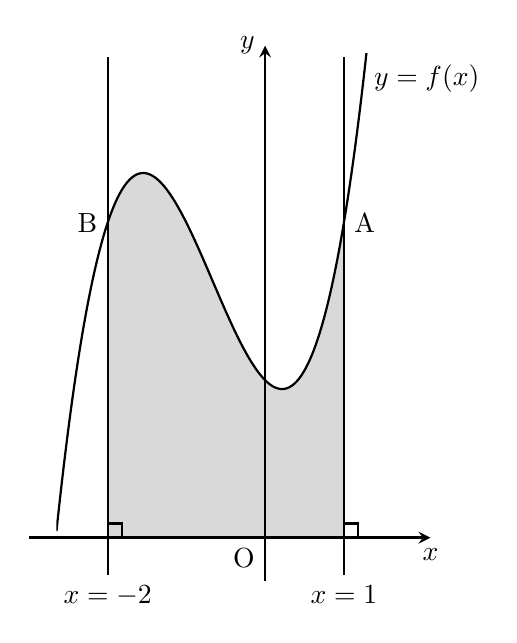
\begin{tikzpicture}[declare function={f(\x)=\x^3 + 2*(\x)^2 - \x + 2;}]

\fill[gray!30]
    (-2,0) -- (-2,{f(-2)}) -- plot[domain=-2:1, samples=120, variable=\t] (\t,{f(\t)}) -- (1,0) -- cycle;

% 좌표축
\draw[-stealth] (-3,0) -- (2.1,0) node[below] {$x$};
\draw[-stealth] (0,-0.55) -- (0,6.25) node[left] {$y$};

% 함수 그래프
\begin{scope}
\clip (-2.65,-0.45) rectangle (1.42,6.15);
\draw[thick]
    plot[domain=-2.65:1.32, samples=160, variable=\t] (\t,{f(\t)});
\end{scope}

% 경계선과 직각 표시
\draw[thick] (1,-0.48) node[below] {$x=1$} -- (1,6.10);
\draw[thick] (-2,-0.48) node[below] {$x=-2$} -- (-2,6.10);
\draw (-2,0) ++(0.18,0) -- ++(0,0.18) -- ++(-0.18,0);
\draw (1,0) ++(0.18,0) -- ++(0,0.18) -- ++(-0.18,0);

% 점과 문자
\node[left] at (-2,{f(-2)}) {$\mathrm{B}$};
\node[right] at (1,{f(1)}) {$\mathrm{A}$};
\node[below left] at (0,0) {$\mathrm{O}$};
\node[right] at (1.25,{f(1.25)}) {$y=f(x)$};
 
\end{tikzpicture}

\end{document}

